\chapter{ニューラルネットを用いた機械学習}
本章では機械学習の中の一つであるニューラルネットについて基本的なことから説明し,次にCNN,GAN,MINEの仕組みについて詳しく説明する.

\section{深層学習}
 深層学習は,\figref{fig:neuron}に示すような生物の脳の神経細胞をモデル化したニューロンを基にして,\figref{fig:tasou}のようにニューロンを多層に結合したモデル(ニューラルネットワーク)を用いる学習法である.個々のニューロン間の結合には重み$\bm{w}$というパラメータが与えられており,$\bm{w}$が更新されていく(学習する)ことで,問題にあった最適解を導く.この重み$\bm{w}$の学習法として,誤差逆伝播法を用いる.誤差逆伝播法は教師信号値$\bm{t}$と出力結果値$\bm{h(x)}$の誤差の大きさを表す損失関数$E$を定義し,$E$に対し各層の$\bm{w}$の微分係数(勾配)を求めることで$\bm{w}$を更新していく.\\
\begin{figure}[htbp]
	\begin{minipage}{0.5\hsize}
		\begin{center}
			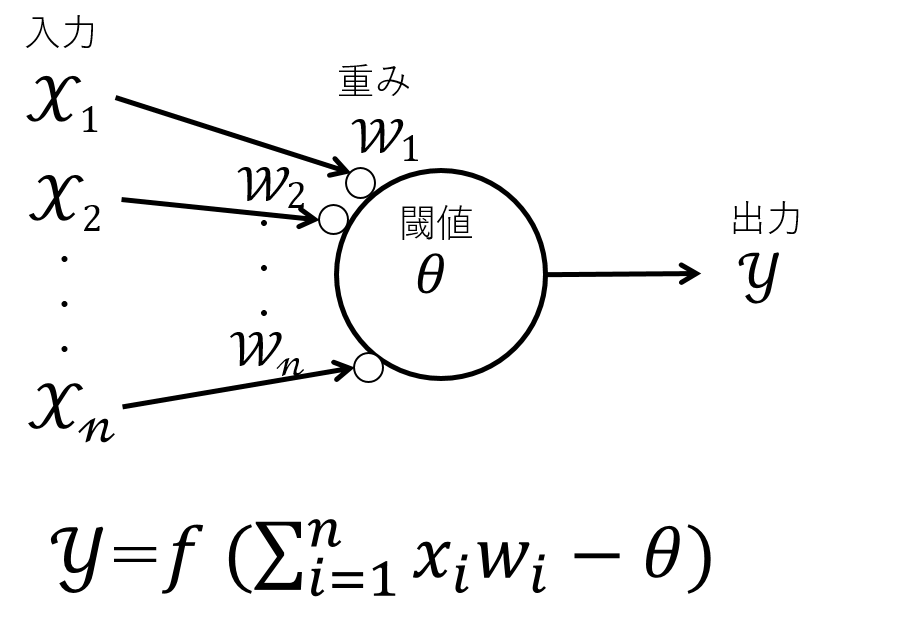
\includegraphics[scale=0.5]{./images/deeplearning/neuron_model.png}
			\caption{ニューロンモデル}
			\label{fig:neuron}
		\end{center}
	\end{minipage}
	\begin{minipage}{0.5\hsize}
		\begin{center}
			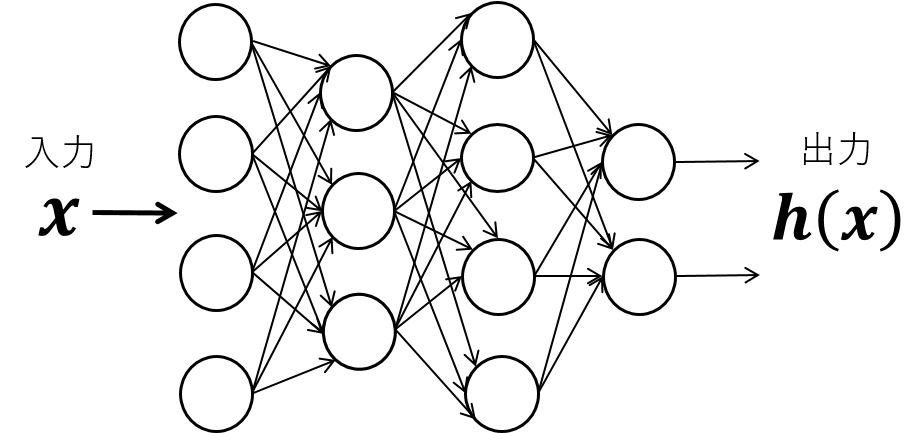
\includegraphics[scale=0.5]{./images/deeplearning/tasou.png}
			\caption{多層パーセプトロン}
			\label{fig:tasou}
		\end{center}
	\end{minipage}
\end{figure}

\section{損失関数と重み最適化}
\subsection{損失関数}
 損失関数$E$は様々な種類があり,一般的によく使われるものとして\eref{eq:loss-crossentropy}~\eref{eq:loss-abs}の,交差エントロピー誤差,平均2乗誤差,平均絶対誤差などがある.
 \begin{eqnarray}
	E &=& -\sum_{k}^{n} t_k log(h_{k}(\bm x)) \label{eq:loss-crossentropy} \\
	E &=& \frac{1}{n}\sum_{k}^{n}{( t_k - h_{k}(\bm x) )^2} \\
	E &=& \frac{1}{n}\sum_{k}^{n}| t_k - h_{k}(\bm x) | \label{eq:loss-abs}
\end{eqnarray}

\subsection{重み最適化}
$\bm{w}$を更新する手法は様々あるが,基本となっているものは\eref{eq:w_new}の勾配降下法であり,損失関数の勾配が減少する方向に学習率$\eta$を乗算した値を加えていくことで$\bm{w}$の最適値を見つけていく.
\begin{eqnarray}
	\label{eq:w_new}
	\bm{w_{t+1}} = \bm{w_{t}} - \eta \frac{\partial E}{\partial \bm{w}}
\end{eqnarray}
\begin{figure}[htbp]
	\begin{center}
		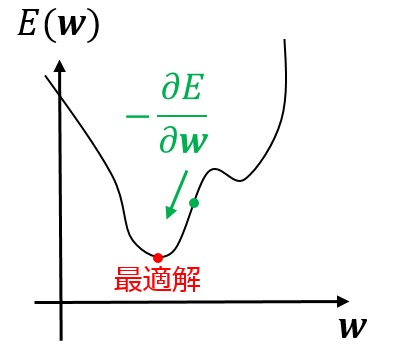
\includegraphics[scale=1]{./images/deeplearning/sgd.png}
		\caption{勾配降下法}
		\label{fig:sgd}
	\end{center}
\end{figure}

\newpage
\subsection{Adam}
Adamは\eref{eq:w_new}を派生させた$\bm w$の更新方法で現在よく用いられている最適化アルゴリズムである\cite{Adam}.
2015年にDiedeik P. Kingmaらが提唱した手法であり,\eref{eq:Adam}のように学習ステップごとに過去の勾配の値から勾配の重みつき平均と重みつき分散を推定している.これにより,更新が多い重みの学習率を低く,更新が少ない重みの学習率を高くするように設定され,学習の収束が早くなることが期待できる.\eref{eq:beta1}, \eref{eq:beta2}における$\beta_1,\beta_2$はハイパーパラメータを表し,実装する側が指定する値である.

\begin{align}
	\label{eq:Adam}
	\bm{w_{t+1}} &= \bm{w_{t}} - \eta \frac{\bm{\hat{m}}} {\sqrt{\bm{\hat{v}}} + \epsilon}\\
	\bm{\hat{m}} &= \frac{\bm{m_{t+1}}}{1-\beta_1^t} \nonumber \\
	\bm{\hat{v}} &= \frac{\bm{m_{t+1}}}{1-\beta_2^t} \nonumber
\end{align}
\vspace{-2zh}
\begin{align}
	\bm{m_{t+1}} &= \beta_1\bm{m_t} + (1-\beta_1) \frac{\partial E}{\partial \bm{w_t}} = (1-\beta_1) \sum_{i=1}^{t} \beta_{1}^{t-i} \bm{m_i} \label{eq:beta1} \\
	\bm{v_{t+1}} &= \beta_2\bm{v_t} + (1-\beta_2) (\frac{\partial E}{\partial \bm{w_t}})^2 = (1-\beta_2) \sum_{i=1}^{t} \beta_{2}^{t-i} \bm{v_i} \label{eq:beta2}
\end{align}


\newpage
\section{畳み込みニューラルネットワーク}
畳み込みニューラルネットワーク(CNN : Convolutional Neural Network)は,人間の視覚野の神経細胞の二つの働きである「画像の濃淡パターンを検出する(特徴抽出)」,及び「物体の位置が変動しても同一の物体であるとみなす(位置ズレの考慮)」を組み合わせたものとなっており,画像分野において高い評価を持つニューラルネットワークとなっている\cite{CNN}.また,入力データのパターンをうまく学習できるという点で,画像だけでなくを様々な問題設定でCNNが広く用いられ,高い精度を出している.

\figref{fig:CNN}は画像分類問題を例にとったCNNのモデルを示している.入力画像は特徴抽出部で特徴が抽出され,その特徴をもとに識別部でパターン分類を行う.特徴抽出部では数層の畳み込み層とプーリング層から構成され,識別部は全結合層から構成されている.
\\
\\

\begin{figure}[htbp]
	\begin{center}
		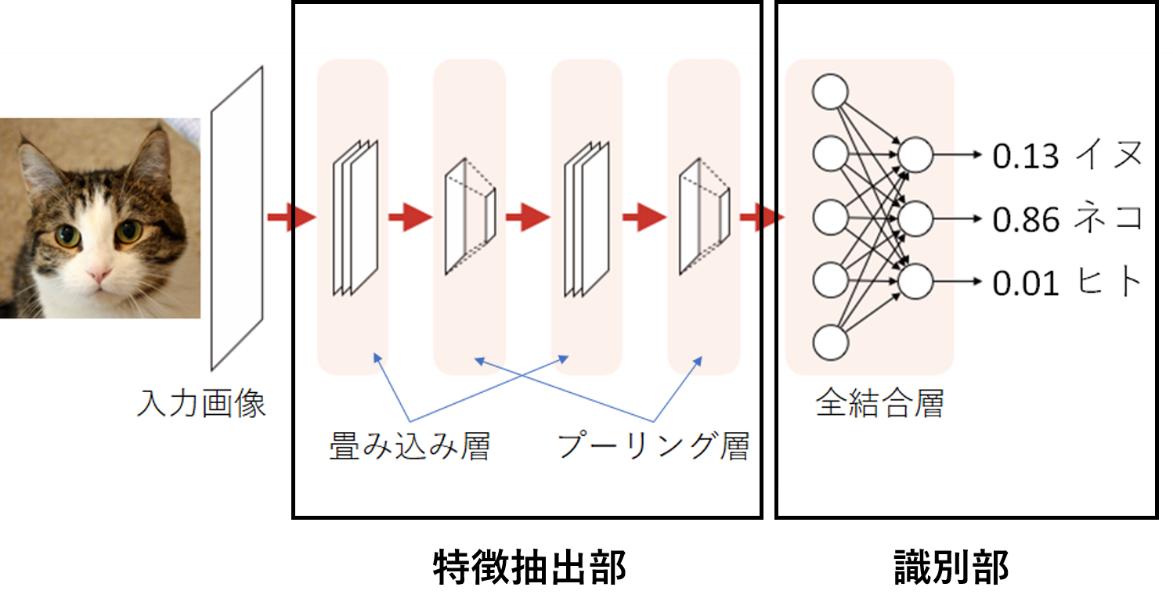
\includegraphics[scale=1.0]{./images/deeplearning/CNN.png}
		\caption{畳み込みニューラルネットワーク}
		\label{fig:CNN}
	\end{center}
\end{figure}

\newpage
\subsection{畳み込み層}
畳み込み層は画像の濃淡パターンを検出するための層に相当する.\figref{fig:convolution}に示すように,入力画像に対し各ピクセル値にフィルタを適用し,フィルタをスライドさせながら画像を圧縮し,特徴マップを作成する.学習時にはフィルタの値が更新される.
\begin{figure}[htbp]
	\begin{center}
		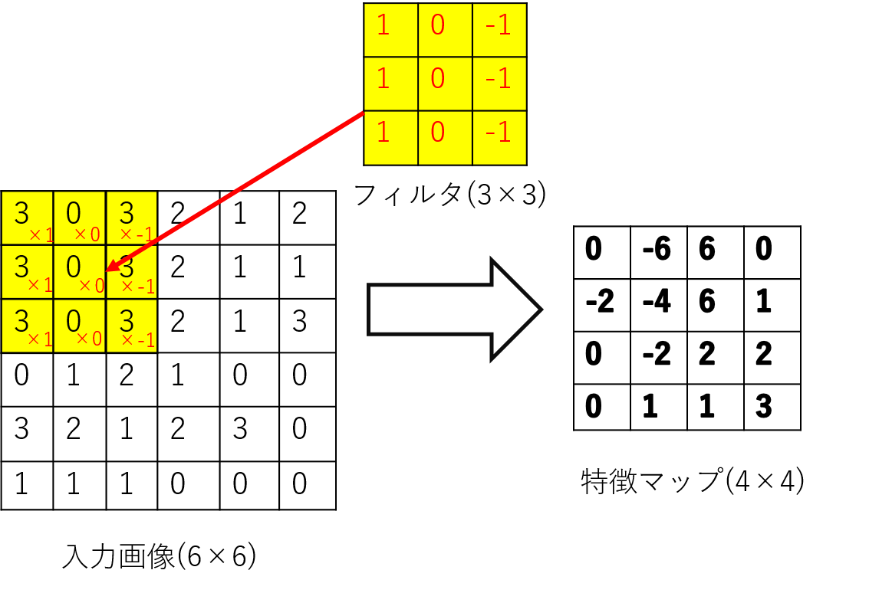
\includegraphics[scale=0.83]{./images/deeplearning/convolution.png}
		\caption{畳み込み}
		\label{fig:convolution}
	\end{center}
\end{figure}
\vspace{-40pt}
\subsection{プーリング層}
プーリング層は位置に対する感度を低くする代わりに,位置変化に対する認識能力を上げるための層に相当する.畳み込み層で得られた特徴マップに対しさらに圧縮をかけることで位置ズレの変化に対応する仕組みとなっている.圧縮のかけ方としては,最大プーリングと平均プーリングがある.\figref{fig:pooling}に示すのは最大プーリング(max pooling)であり,特徴マップの小領域の中から最大のピクセル値を得る操作となっている.対して平均プーリング(average pooling)は小領域の中の値を平均した値を得る操作となる.プーリング層においては学習時に更新されるパラメータは存在しない.

\begin{figure}[htbp]
	\begin{center}
		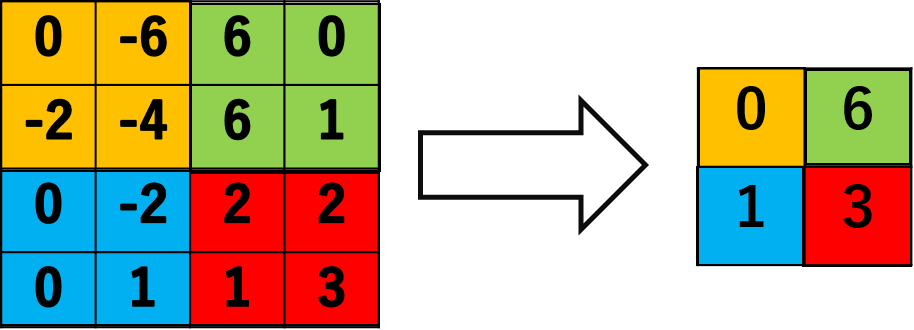
\includegraphics[scale=0.293]{./images/deeplearning/pooling.png}
		\caption{最大プーリング}
		\label{fig:pooling}
	\end{center}
\end{figure}

\newpage
\subsection{全結合層と活性化関数}
全結合層は,特徴抽出部から得られた特徴マップの値を入力とし,\figref{fig:tasou}のような多層パーセプトロンのニューラルネットワークによりパターン分類が行われる層である.最後のニューロンの出力数は問題設定に応じて変更される.分類問題の場合は分類したいクラス数であったり,画像生成問題の場合は画像のピクセルサイズ分の出力を持ったりなどをする.

各層のニューロンの出力値は活性化関数が通された後の値となっている.これは,ニューロンの出力が線形であるため,多層パーセプトロンと等価な1層のパーセプトロンの対が必ず存在してしまうことを避けるためである.活性化関数には,ランプ関数(ReLU),ソフトマックス関数,シグモイド関数などといったものが存在する.


\subsubsection{Relu関数}
中間層のニューロンの出力を非線形にするためによく使用されている関数である.非負の値を出力する.
\begin{eqnarray}
	f(x) = max(0, x)
\end{eqnarray}

\subsubsection{ソフトマックス関数}
ニューロンの出力を確率として扱う場合に使用される関数である.分類問題において最終層のニューロンの活性化関数として使用され,\eref{eq:softmax}で表される.
$a_k$は$k$番目のニューロンの出力値であり,$n$は最終層のニューロンの出力数である.
\begin{eqnarray}
	f_k(a_k) = \frac{e^{a_k}}{\displaystyle \sum_{i=1}^{n} e^{a_i}} \label{eq:softmax}
\end{eqnarray}

\subsubsection{シグモイド関数}
出力値を0~1に収める関数である.ニューロンの出力値を非線形したいときや,確率とみなしてマルチクラス分類をする際にも使用されている.
\begin{eqnarray}
	f(x) = \frac{1}{1+ e^{-x}}
\end{eqnarray}


\newpage
\section{敵対生成ネットワーク}
敵対生成ネットワーク(GAN : Generative Adversarial Network)は,学習データと似たような新しいデータを生成する生成モデルの一種であり,言い換えれば生成データの分布を学習データの分布に近づけていくように学習するモデルである.GANの構造を\figref{fig:GAN}に示す.GANは\figref{fig:GAN}に示すように,生成器(Generator)と識別器(Discriminator)から構成され,Generatorはランダムノイズからオリジナルと似たデータを生成し,Discriminatorは入力されるデータがGeneratorによって作られたデータか,それともオリジナルのデータかの識別を行う.これら二つのモデルが互いを見抜く・騙すように学習するため,十分に学習が進むとGeneratrはオリジナルのデータと見分けがつかないようなデータを生成するようになる.\\
\begin{figure}[htbp]
	\begin{center}
		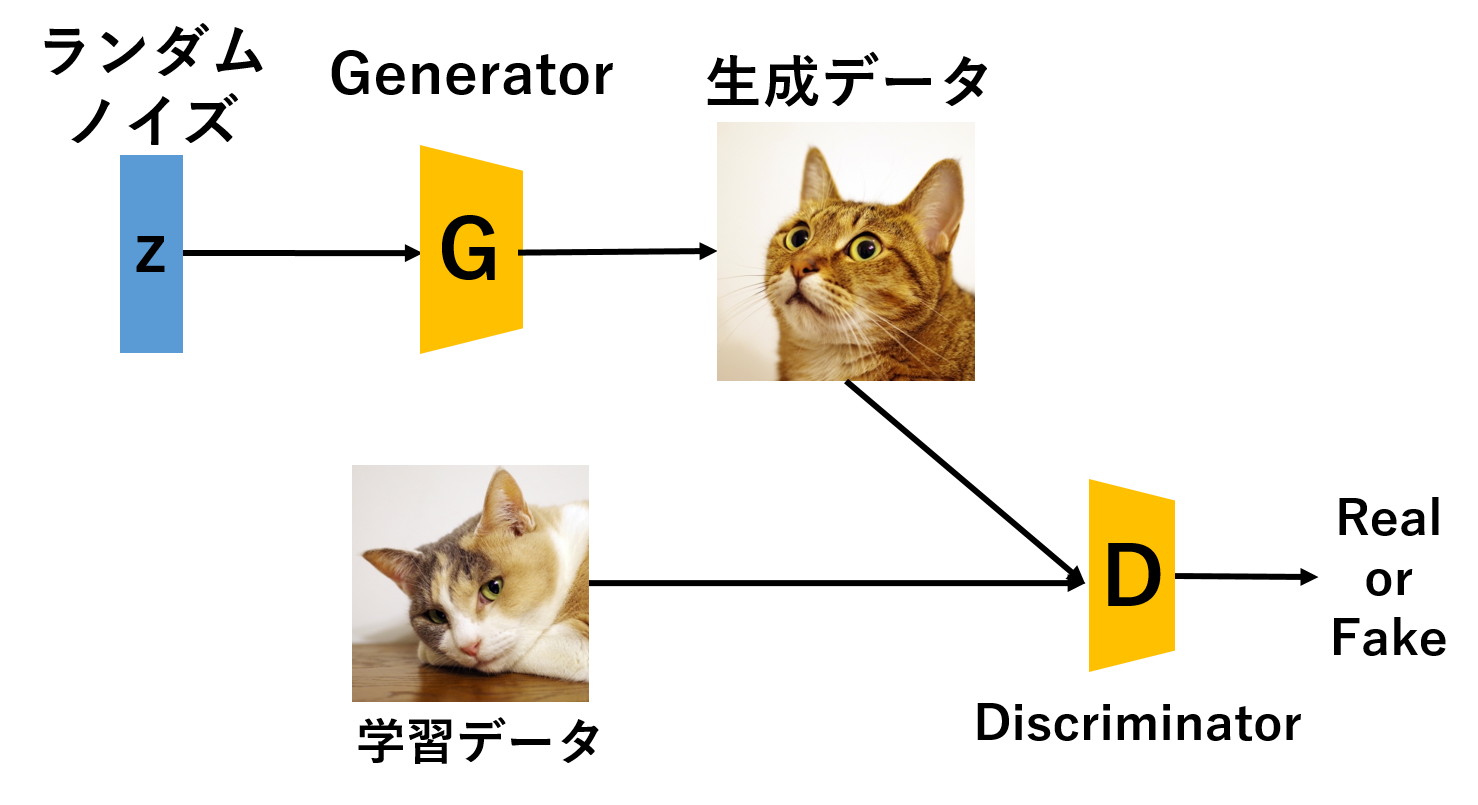
\includegraphics[scale=0.6]{./images/deeplearning/GAN.png}
		\caption{敵対生成ネットワーク(GAN)}
		\label{fig:GAN}
	\end{center}
\end{figure}

\newpage
\subsection{GANの損失関数}
具体的に評価関数を導入して学習を行う場合,\eref{eq:minimax}に関して,Discriminatorに対して最大化,Generatorに対して最小化するミニマックスゲームを考えればよい\cite{GAN}.
\begin{eqnarray}
	min_G max_DV(G, D) = \mathbb E_{\bm x \sim p_r(\bm x)}[{\rm log}D(\bm x)] + \mathbb E_{\bm z \sim p_z(\bm z)}[1 - {\rm log}D(G(\bm z))] \label{eq:minimax}
\end{eqnarray}
\eref{eq:minimax}において,$\bm x$はオリジナルデータ,$p_r(\bm x)$はオリジナルデータの確率分布,$\bm z$はランダムノイズ,$p_z(\bm z)$はランダムノイズの確率分布を示す.
この時,$D$がオリジナルのデータを正しく判定できれば${\rm log}D(\bm x)$が大きくなり,$D$が$G$の生成データをオリジナルのデータと誤って判定すると${\rm log}(1-D(G(\bm z)))$が小さくなる.

\subsection{GANの最適解}
\eref{eq:minimax}において,$\bm z \sim p_z(\bm z)$から$G$が生成するデータの分布を$p_g(\bm x)$とし,$V(G, D)$を書き直すと,
\begin{eqnarray}
	V(G, D) = \int_{\bm x} \{p_r(\bm x) {\rm log}D(\bm x) + p_g(\bm x) {\rm log}(1-D(\bm x)) \} \bm{dx}\label{eq:minmax}
\end{eqnarray}
となる.Discriminatorの最適解は$V(G, D)$を最大化することであるため,積分の中身の最大化をすればよい.よって中身を$D(\bm x)$に関して微分し,その時の導関数が0になる$D(\bm x)$を$D^*(\bm x)$とすると,\eref{eq:dis_opt}となる.
\begin{eqnarray}
	D^*(\bm x) = \frac{p_r(\bm x)}{p_r(\bm x) + p_g(\bm x)}\label{eq:dis_opt}
\end{eqnarray}
またこのとき,Generatorの最適化を考える.\eref{eq:dis_opt}の右辺を\eref{eq:minmax}に代入し式を整理すると,\eref{eq:jensengan}となる.
\begin{eqnarray}
	V(G, D) = 2D_{JS}(p_r||p_g)-\rm log4 \label{eq:jensengan}
\end{eqnarray}
\eref{eq:jensengan}を最小化することは,Jensen-Shannonダイバージェンスの最適化と等しく,$p_g = p_r$のときに最小値$- \rm log4$をとる.


\subsection{Wasserstein GAN}
 二つの確率分布の距離として定義したJensen-Shannonダイバージェンスを損失関数としたとき,関数に不連続な箇所が見受けられ,勾配が求められないという問題があった\cite{wgan}.そこで,関数に連続性を持たせるために新たにWasserstein距離を二つの確率密度関数の距離を測る指標として導入し,それを用いたGANをWasserstein GAN(WGAN)と言う.

\subsubsection{Wasserstein距離}
Wasserstein距離は,\eref{eq:wasserstein}で与えられる
\begin{eqnarray}
	W(p_r, p_g) = \underset{\gamma \sim \prod(p_r, p_g)}{\rm{inf}} \mathbb E_{(\bm x, \bm y) \sim \gamma} [||\bm x - \bm y||] \label{eq:wasserstein}
\end{eqnarray}


$\prod(p_r, p_g)$は$p_r$と$p_g$の同時分布を示し,$\gamma(\bm x, \bm y)$は$p_r$のある地点$\bm x$を$p_g$のある地点$\bm y$に移動させる量である.その量にノルム$||\bm x - \bm y||$をかけたものをコストとして定義し,コストを最小にしたものがWasserstein距離である.この関数はどの点においても連続になるため,勾配がすべての点で存在する.
また\eref{eq:wasserstein}はKantrovich-Rubinstein双対性を用いて,\eref{eq:wasserstein2}に変形できる.
\begin{align}
	W(p_r, p_g) &= \frac{1}{K}\underset{||f||_L \leq K}{\rm sup} \mathbb E_{\bm x \sim p_r}[f(\bm x)] - \mathbb E_{\bm x \sim p_g}[f(\bm x)] \nonumber \\
	&= \frac{1}{K}\underset{||D||_L \leq K}{\rm sup} \mathbb E_{\bm x \sim p_r}[D(\bm x)] - \mathbb E_{\bm z \sim p_z}[D(G(\bm z))] \label{eq:wasserstein2}
\end{align}
 

\subsubsection{損失関数}
 \eref{eq:wasserstein2}からWasserstein距離を求めるためには最大化問題を解かなければならない.Wasserstein GANではこの問題をDiscriminatorが担い,より正確なWasserstein距離を求めようとする.対してGeneratorはDiscriminatorで求めたWasserstein距離を最小化するように学習を行う.つまり,Discriminator損失関数は\eref{eq:wasserstein2}である.
一方Generatorの損失関数は\eref{eq:wasserstein2}をGeneratorが持つ学習パラメータ$\theta$で微分した\eref{eq:wasserstein3}とすることで,$W(p_r, p_g)$を最小化すればよいことがわかる.\eref{eq:wasserstein3}における$M$はバッチサイズを示す.
\newpage
\begin{align}
 	\frac{\partial W(p_r, p_g)}{\partial \theta} &= - \mathbb E_{\bm z \sim p_z}[\frac{\partial D(G(\bm z))}{\partial \theta}]\nonumber \\
 	&\simeq -\frac{1}{M} \sum_{m=1}^{M}\frac{\partial}{\partial \theta}D(G(\bm z_m)) \label{eq:wasserstein3}
\end{align}


\subsubsection{Gradient Penalty}
WGANには\eref{eq:wasserstein2}からわかるようにDiscriminatorの制約条件として$K-$リプシッツ連続の関数であることが前提である.この制約から\cite{wgan}ではDiscriminatorの学習パラメータの値が$[-c, c](cは任意値)$になるようにクリッピングを行っている.しかしクリッピングでは勾配が爆発したり消失したりするのに加え,学習の収束が遅いという欠点があった.そこで,Ishaanらによる勾配に制約を設けたWGAN-gpが提案されている\cite{wgan-gp}.

WGAN-gpでは,「最適化されたWGANのDiscriminatorは$p_r, p_g$下のほぼすべての点において大きさ1の勾配持つ」という性質を利用して,Discriminatorの損失関数の項に,
\begin{gather}
	\lambda \mathbb E_{\bm{\hat x} \sim p_{\hat x}}[(|\frac{\partial D(\bm{\hat x})}{\partial \bm{\hat x}}| - 1)^2]\nonumber
\end{gather}
を加えたものを新たに損失関数として定義する.ここで,$\lambda$はハイパーパラメータであり,$\bm{\hat  x}$は
\begin{gather}
	\bm{\hat x} = \epsilon \bm x + (1 - \epsilon) \bm{\tilde x} \nonumber \\
	\epsilon \sim U[0, 1], \quad  \bm x \sim p_r, \quad \bm{\tilde x} \sim p_g \nonumber
\end{gather}
で表され,$U[0, 1]$は0~1の一様分布に従う乱数を示す.


\newpage
\section{ニューラルネットによる相互情報量の推定と最大化}
\subsection{相互情報量}
相互情報量は二つの確率変数を測る尺度であり,二つの確率変数を$X,Y$とすると \eref{eq:mutual-information}で定義される.
\begin{eqnarray}
	I(X;Y) &=& H(X) - H(X|Y) \label{eq:mutual-information}\\
	H(X) &=& -\mathbb E_{P(X)}[{\rm log}P(x)] \nonumber \\
	H(X|Y) &=& -\mathbb E_{P(X), P(Y)}[{\rm log}P(X|Y)] \nonumber
\end{eqnarray}
$H$は情報量エントロピーを示し,$H(X|Y)$は条件付エントロピーを表す.さらに\eref{eq:mutual-information}を変形していくと,
\begin{eqnarray}
	I(X;Y) &=& \mathbb E_{P(X), P(Y)}[{\rm log}P(X|Y)] - E_{P(X)}[{\rm log}P(X)] \nonumber \\
	&=& \mathbb E_{P(X), P(Y)}[{\rm log}P(X|Y)P(X)] \nonumber \\
	&=& \mathbb E_{P(X), P(Y)}[{\rm log}P(X, Y)P(X)P(Y)] \nonumber \\
	&=& D_{KL}(P(X, Y)||P(X)P(Y)) \nonumber \\
	&=& \underset{T:\Omega \rightarrow \mathbb R}{\rm sup}\mathbb E_{P(X,Y)}[T] - {\rm log}(\mathbb E_{P(X), P(Y)}[e^T]) \label{eq:mutual_estimation}
\end{eqnarray}
と表せる.

\subsection{Mutual Information Neural Estimation}
相互情報量は二つの確率変数間の依存関係を測る指標であるが,一般的に計算するのが難しい.そこでニューラルネット(NN)を用いて相互情報量を推定する方法がMutual Information Neural Estimation(MINE)である\cite{MINE}.

\eref{eq:mutual_estimation}の関数$T$をパラメータ$\theta$を持つNNで表現された関数$T_{\theta}$と考える.このとき,相互情報量は,\eref{eq:mine}となる
\begin{eqnarray}
	I(X;Y) \geq I_{\Theta}(X;Y) = \underset{\theta \in \Theta}{\rm sup}\: \mathbb E_{P(X,Y)}[T_{\theta}] - {\rm log}(\mathbb E_{P(X), P(Y)}[e^{T_{\theta}}]) \label{eq:mine}
\end{eqnarray}
\eref{eq:mine}における期待値は$P(X, Y), P(X)P(Y)$からのサンプリングを用いて計算され,上限を求める際は勾配法による最大化を行う.NNは表現力に優れているため,任意の精度で相互情報量を近似することが可能となる.プログラムで実装する場合は\eref{eq:mine}の最大化問題を式全体にマイナスを掛けることにより最小値問題に置き換え,下限を求めるために勾配降下法を用いる.

\subsection{Mutual information estimation and maximization}
MINEの枠組みに従って得られる相互情報量を最大化し,確率変数$X, Y$に従属関係を持たせる場合を考える.Yの確率変数をパラメータ$\omega$に従うNN,$Y_{\omega}=F_{\omega}(X)$から得られる確率変数として置き換える.このとき確率変数$X, Y_{\omega}$の相互情報量を最大化するためには,\eref{eq:infomax}を解くことに等しい.
\begin{eqnarray}
	\underset{\theta, \omega}{\rm argmax}\: I_{\theta}(X;F_{\omega}(X)) \label{eq:infomax}
\end{eqnarray}
ここで,相互情報量の推定と最大化にNNを用いて最適化を行っていることから,目的関数を一つで表し両者の最適化を同時に行う.$f_{\omega}, C_{\omega}, D_{\theta}$を任意のNNとし,$F_{\omega} = f_{\omega}\circ C_{\omega}$,$T_{\theta, \omega} = D_{\theta} \circ C_{\omega}$のように組み合わせる.このとき相互情報量の推定と最大化を行うための目的関数\eref{eq:infomax}は,Jensen-Shannonダイバージェンスを用いて\eref{eq:deepinfomax}と表すことができる\cite{deepinfomax}.
\begin{eqnarray}
	 \underset{\theta, \omega}{\rm argmax} \: \mathbb E_{P(X, F_{\omega}(X)))} [-{\rm sp}(-T_{\theta, \omega}(x, F_{\omega}(x)))] - \mathbb E_{P(X), F_{\omega}(X)} [{\rm sp}(T_{\theta, \omega}(\bar x, F_{\omega}(x)))] \label{eq:deepinfomax}
\end{eqnarray}
\eref{eq:deepinfomax}における$x, \bar x$はそれぞれ異なる入力サンプルで,sp$(z)$ = log$(1+e^z)$である.プログラムで実装する場合は\eref{eq:deepinfomax}にマイナスを掛け最小化問題にすることで勾配降下法を用いる.
